\documentclass[10pt]{extarticle}
\usepackage[sfdefault]{FiraSans}
\usepackage[T1]{fontenc}
\usepackage[utf8]{inputenc}
\usepackage{adjustbox}
\usepackage{algorithm}
\usepackage{algorithmic}
\usepackage{amsfonts}
\usepackage{amsmath}
\usepackage{amssymb}
\usepackage[style=apa]{biblatex}
\addbibresource{references.bib}
\usepackage{booktabs}
\usepackage{breqn}
\usepackage{enumitem}
\usepackage{float}
\usepackage{geometry}
\usepackage{graphicx}
\usepackage{hyperref}
\usepackage{lipsum}
\usepackage{listings}
\usepackage{longtable}
\usepackage{multirow}
\usepackage{pdfpages}
\usepackage{pgfgantt}
\usepackage{setspace}
\usepackage{subcaption}
\usepackage{tabularx}
\usepackage{tikz}
\usetikzlibrary{positioning,shapes.geometric,arrows.meta,fit}
\usepackage{xcolor}

\DeclareLanguageMapping{english}{english-apa}

\geometry{letterpaper, left=1in, right=1in, top=1in, bottom=1in,}

\definecolor{primary}{RGB}{0,120,215}
\definecolor{secondary}{RGB}{255,87,34}
\definecolor{background}{RGB}{245,245,245}
\definecolor{blue}{RGB}{0,62,126}

\pagecolor{background}

\hypersetup{colorlinks=true, linkcolor=primary, filecolor=secondary, urlcolor=primary, citecolor=black}

\AtBeginBibliography{\hypersetup{urlcolor=black}}

\setstretch{1.15}

\setlength{\bibhang}{0.5in}
\setlength\bibitemsep{1.5\itemsep}

\setlength{\parindent}{0pt}
\setlength{\parskip}{1em}

\nocite{*}

\begin{document}

\newcommand{\mytitlepage}[2]{
    \thispagestyle{empty}

    \begin{tikzpicture}[remember picture, overlay]
        \node [inner sep=0pt] at (current page.center) {#1}; { \node [ anchor=center, inner sep=1.25cm, rectangle, fill=blue!70!white, fill opacity=0, text opacity=1, minimum height=0.2\paperheight, minimum width=\paperwidth, text width=0.8\paperwidth, font=\fontfamily{pnc}\selectfont ] at (current page.center) {#2}; } \node [anchor=south east, outer sep=3pt] at (current page.south east) {
\includegraphics[width=0.33\paperwidth]{logo.png}};
    \end{tikzpicture}

    \newpage
}

{ \mytitlepage{\includegraphics[width=\paperwidth]{background.png}}
    {
        \centering
        \fontfamily{phv}
        \vspace{-200pt} % move title up
        { \Huge
            \bfseries

            \begin{center}
                DeepSleepNet \\
                A Deep Learning Approach to Enhancing Sleep Quality Analysis and Prediction in IoT-Enabled Devices
            \end{center}

            \par
        }
        \vspace{8pt}
        { \Large
            \bfseries

            Final Report

            \par
        }
        \vspace{24pt}
        {
            \begin{center}
                \begin{tabular*} {\textwidth}{@{\extracolsep{\fill}}c c c}
                    {\LARGE Jonathan Agustin} & {\LARGE Alec Anderson} & {\LARGE Brandon Smith}
                \end{tabular*}
            \end{center}
        }
    }
}

\pagenumbering{arabic}

\begin{center}
    {\LARGE \textbf{DeepSleepNet}} \\
    {\large \textbf{A Deep Learning Approach to Enhancing Sleep Quality Analysis and Prediction in IoT-Enabled Devices}}
\end{center}

\section{Abstract}

We explore sleep quality prediction by combining Long Short-Term Memory (LSTM) networks with machine learning techniques, using data from Fitbit devices. It aims to improve the accuracy of sleep quality metrics from wearable technology. The research involves preprocessing, data analysis, and feature engineering to build models that predict sleep quality and identify sleep behavior patterns. This approach shows how deep learning and statistical models can work together to analyze health data from IoT devices, contributing to personalized health tracking.

\textbf{Keywords:} Sleep Quality, LSTM, Machine Learning, Fitbit Data, Health Informatics.

\section{Introduction}

\subsection{Problem Motivation}

Sleep plays a crucial role in health, affecting cognitive performance, mood, metabolism, and immune function. However, monitoring sleep quality often requires polysomnography, which is expensive and invasive. Wearable devices like Fitbit offer a simpler way to track sleep, providing data on sleep duration, restlessness, and stages. Despite the potential of LSTM networks for time-series data, their use with machine learning for sleep data analysis is limited. This project aims to combine LSTM networks with machine learning to improve sleep health understanding and interventions.

\subsection{Research Gap}

Wearable technology has made it easier to collect sleep data, but the combination of LSTM networks and machine learning in sleep quality prediction needs more exploration. LSTMs can analyze sequential data, while traditional machine learning offers feature extraction and interpretation. This research gap suggests a need for studies that integrate these methods to understand sleep better and improve health outcomes.

\section{System Design}

\subsection{Sensors}
\begin{itemize}
    \item \textbf{Location:} Worn on the user's wrist.
    \item \textbf{Type:} Multi-sensor Fitbit device with motion detection (3-axis accelerometer) and heart rate monitoring (optical heart rate monitor).
    \item \textbf{Limitations:} Sensors may have limited accuracy and are dependent on proper user wear. They may also be affected by user movement and environmental factors.
\end{itemize}

\subsection{Edge Processing}
\begin{itemize}
    \item \textbf{Computation on the Edge:} Basic preprocessing such as filtering raw data to detect sleep stages and restlessness.
    \item \textbf{Edge Device Requirements:} Sufficient computational power and memory for real-time data processing and temporary storage.
\end{itemize}

\subsection{Networking}
\begin{itemize}
    \item \textbf{Device Connection:} Fitbit device connects to a smartphone or Wi-Fi network.
    \item \textbf{Messaging Protocol:} Uses Bluetooth Low Energy (BLE) for syncing with the smartphone app and HTTPS for uploading data to the cloud.
\end{itemize}

\subsection{Data Storage and Processing}
\begin{itemize}
    \item \textbf{Tools and Storage Systems:} Cloud-based storage (e.g., AWS S3) and computing services (e.g., AWS EC2).
    \item \textbf{Scalability Management:} Auto-scaling services to manage increasing user load.
    \item \textbf{Machine Learning Insights Production:} Data is processed and features engineered in the cloud. Machine learning models are trained to predict sleep scores and classify sleep stages.
\end{itemize}

\subsection{Machine Learning Tasks}
\begin{itemize}
    \item \textbf{Deep Learning:} An LSTM network predicts the overall sleep score from time series data.
    \item \textbf{Time Series Prediction:} A traditional machine learning algorithm, such as Random Forest, classifies data into deep sleep and restlessness stages.
\end{itemize}


\begin{tikzpicture}[
    node distance=1.5cm,
    auto,
    block/.style={
        rectangle,
        draw,
        text width=6em,
        align=center,
        rounded corners,
        minimum height=3em
    },
    line/.style={
        draw,
        -{Latex[length=2.5mm]}
    }
]

% Nodes
\node[block] (sensor) {Sensors};
\node[block, below=of sensor] (edge) {Edge Processing};
\node[block, below=of edge] (network) {Networking};
\node[block, below=of network] (storage) {Data Storage};
\node[block, below=of storage] (processing) {Data Processing};
\node[block, below=of processing] (ml) {Machine Learning};

% Edges
\path[line] (sensor) -- (edge);
\path[line] (edge) -- (network);
\path[line] (network) -- (storage);
\path[line] (storage) -- (processing);
\path[line] (processing) -- (ml);

% Annotations
\node[fit=(sensor) (edge) (network) (storage) (processing) (ml), draw, dashed, inner sep=0.5cm, label=above:IoT System Design] (system) {};

\end{tikzpicture}

\section{Dataset and Preprocessing}

\subsection{Dataset Description}

The dataset used in this research originates from Fitbit devices, renowned for their capability to track a lot of health-related metrics such as physical activity, heart rate, and notably, sleep patterns. Our investigation primarily concentrates on the sleep data amassed by these devices, offering an extensive view of user sleep behaviors over prolonged durations.

The overall sleep score is derived from a combination of several key metrics: (i) the duration score, assessing the total amount of sleep obtained; (ii) the revitalization score, evaluating the participant's sense of refreshment upon awakening, determined by factors such as breathing disruptions and sleeping heart rate; and (iii) the composition score, which accounts for the distribution of various sleep stages throughout the night. Additionally, other sleep-related parameters are tracked, including the resting heart rate, the time spent in the deep sleep stage, and restlessness, which reflects the frequency of the participant's movements, such as tossing and turning, during sleep.

\subsection{Preprocessing}

Our preprocessing pipeline includes handling missing values with forward fill, encoding categorical variables, and standardizing features to prepare the dataset for machine learning analysis.

\subsection{Missing Values}

Missing values pose a considerable challenge to the reliability and validity of data-driven projects. Various reasons contribute to missing data, such as human error, equipment failure, or participant withdrawal. No matter the cause, omitting records with missing entries risks compromising the representativeness and generalizability of the analyzed dataset. Instead, filling missing values with informed estimates enables continued inclusion of affected samples in the dataset, preserving statistical power and reducing bias.

We use forward fill imputation, where missing entries are replaced with the immediately preceding non-null observation. This strategy assumes that consecutive data points show a level of autocorrelation, allowing the substitution of missing values with plausible approximations based on historical records.

\subsection{Categorical Variables}

Machine learning algorithms typically rely on numerical inputs, posing difficulties when confronted with categorical variables. Encoding categorical variables allows translation of nominal labels into quantitative representations compatible with computational routines. Among the many encoding strategies, label encoding stands out for its simplicity and wide applicability.

Label encoding assigns unique integer codes to each discrete category within a categorical variable. Zero denotes the reference category, but incremental integers symbolize ascending categories. Applying this scheme makes sure each encoded value remains different from alternative categories, preventing ambiguity in interpretation and maintaining ordinality whenever applicable.

Formally, let \(X\) represent a categorical variable with cardinality \(\left|X\right|\), and \(k\) denote the label encoding function mapping each category onto a unique integer. Then, label encoding can be expressed as:

\[
f_{label}: X \rightarrow \{0, \ldots , \left|X\right|\}
\]

where

\[
f_{label}(x) = k(x)
\]

Label encoding translates categorical features into numerical formats admissible for machine learning algorithms, getting around obstacles imposed by qualitative data structures and giving practitioners versatile tools for integrating disparate data modalities.

\subsection{Continuous Features}

Continuous features often exhibit varying scales and distributions, complicating comparisons between variables and hampering efficient learning of inherent patterns concealed beneath heterogeneous magnitudes. Standardization addresses this concern by equalizing the spread and location of each feature, rendering them commensurable and enhancing the efficacy of machine learning algorithms.

Standardization centers the distribution of each continuous feature around its mean \(\mu{}\) and scales its variance (\(Var\)) to unity. Mathematically, standardization corresponds to z-scoring, defined as:

\[
z = \frac{(x - \mu)}{\sqrt{Var}}
\]

where \(x\) denotes the original measurement and \(z\) symbolizes the transformed feature. Normalizing the distribution of continuous features bolsters the stability and robustness of machine learning models, promotes faster convergence rates, and reduces sensitivity to initialization hyperparameters.

Executing judicious preprocessing techniques, such as handling missing values, transforming categorical variables, and standardizing continuous features, fortifies the integrity and consistency of the dataset, amplifying the likelihood of deriving insightful conclusions and cultivating dependable machine learning models. The subsequent sections elucidate the application of these preparatory measures to the Fitbit-derived sleep score dataset, setting the stage for more intricate investigations and nuanced analyses.

\section{Exploratory Data Analysis (EDA)}

\subsection{Overall Sleep Score}

The overall sleep score is a composite metric calculated by Fitbit, summarizing the quality of sleep on a scale from 0 to 100. Higher scores indicate better sleep quality, incorporating factors such as sleep duration, restlessness, and time spent in various sleep stages. Descriptive statistics for the overall sleep score reveal the average sleep quality experienced by participants and the range of sleep quality within the dataset.

\section{Feature Engineering}

We focus on enhancing our dataset by creating new features that can improve the performance of our machine learning models. One key technique we employ is the generation of lagged features for various variables, which helps in capturing temporal patterns within the data.

\subsection{Creating Lagged Features}

To account for the temporal dependencies inherent in sleep data, we introduce lagged features as a fundamental part of our feature engineering approach. These features, which are time-shifted versions of existing variables, are designed to incorporate historical information into the predictive models, enabling them to leverage past data to forecast future sleep quality.

We generate lagged features for critical variables such as sleep duration, restlessness, and sleep stages, extending up to seven days back. This inclusion of historical context lets our models recognize and use temporal patterns in sleep data, enhancing their predictive capabilities. The determination of the best lag intervals and the quantity of lagged features to include is achieved through exploratory data analysis and empirical validation, aiming to strike an ideal balance between the complexity of the model and its predictive accuracy.

\subsection{Injecting Noise to Increase Robustness}

To mitigate overfitting and to better reflect the inherent variability in sleep data, we implement a controlled noise augmentation strategy. This involves perturbing selected features with Gaussian noise, characterized by a zero mean and a standard deviation of 0.02. The features subjected to this augmentation include sleep duration metrics, resting heart rate, and measures of restlessness, along with their respective lagged versions up to seven days before. This augmentation aims to improve the models' generalization by preventing them from overly fitting to the nuances of the training dataset, thus enhancing their performance on unseen data.

\subsection{Implications for Sleep Quality Prediction}

The advanced feature engineering techniques used in our study—lagged feature generation and controlled noise injection—play a pivotal role in bridging the gap between raw sleep data and actionable predictive insights. By incorporating temporal dynamics and enhancing model robustness, we equip our models with tools to navigate the complexities of sleep behavior.

These strategies not only improve the accuracy of sleep quality predictions but also contribute to a deeper understanding of the factors influencing sleep. The insights gleaned from our models have the potential to inform personalized sleep interventions, guiding individuals towards improved sleep hygiene and better health outcomes.

Our feature engineering approach exemplifies the synergy between domain knowledge and machine learning knowledge. By thoughtfully crafting features that reflect the temporal and stochastic nature of sleep, we set a new benchmark for predictive modeling in the realm of sleep science. This endeavor not only advances the field of sleep quality prediction but also underscores the importance of innovative feature engineering in unlocking the full potential of wearable device data for health tracking and intervention.

\section{LSTM Model Development}

\subsection{Architecture}

The architecture of our Long Short-Term Memory (LSTM) model is meticulously designed to harness the full potential of time-series data derived from Fitbit devices, capturing the intricate temporal dynamics inherent in sleep patterns. This section digs into the architecture of our LSTM model, elucidating the strategic layer choices and their underlying reasoning, which collectively aim to optimize the model's predictive performance in assessing sleep quality.

\subsubsection{Bidirectional LSTM Layers}

At the core of our model architecture are the Bidirectional LSTM layers, which represent a significant advancement over traditional unidirectional LSTMs. By processing the time-series data in both forward and backward directions, these layers can capture dependencies and patterns that may be overlooked when the data is traversed in a single direction. This dual processing mechanism is advantageous in sleep data, where both preceding and later sleep metrics can offer valuable insights into the quality of a given night's sleep. Including Bidirectional LSTM layers underscores our commitment to leveraging deep learning innovations to enhance the model's sensitivity to temporal correlations within the dataset.

\subsubsection{BatchNormalization Layers}

To further bolster the model's efficiency and convergence speed, we incorporate BatchNormalization layers following each LSTM layer. These layers normalize the activations from the previous layer, making sure the distribution of inputs to later layers remains stable throughout the training process. By mitigating the internal covariate shift phenomenon, BatchNormalization layers help with the use of higher learning rates, accelerating the training phase without compromising the stability of the gradient descent process. This feature is crucial in sleep quality prediction, where the model must navigate through vast, multidimensional datasets to identify salient patterns and trends.

\subsubsection{Dropout Layers}

Recognizing the risk of overfitting in deep learning models, especially when dealing with relatively limited datasets, we strategically integrate Dropout layers into our architecture. These layers randomly deactivate a subset of neurons during the training phase, effectively introducing regularization by preventing the model from becoming overly reliant on any specific set of features. This approach encourages the development of a more generalized model capable of performing robustly on unseen data. The Dropout layers play a pivotal role in enhancing the model's generalization capabilities, making sure the predictive insights generated are not only accurate but also broadly applicable.

\subsubsection{Dense Layers and Activation Functions}

The culmination of our LSTM model architecture is Dense layers, which  integrate the high-level features extracted by the LSTM layers into final predictions regarding sleep quality. The activation function used in the output layer is meticulously selected based on the prediction task; for regression tasks, a linear activation function is used, while classification tasks may leverage softmax or sigmoid functions. This layer configuration makes sure the model's output is appropriately scaled and interpretable, directly aligning with the goals of sleep quality assessment.

\subsection{Compilation and Training}

The compilation and training phase of our LSTM model is a critical juncture where theoretical design transitions into practical application, enabling the model to learn from the intricacies of sleep data. This process is meticulously orchestrated to make sure the model's architecture is not only theoretically sound but also almost effective in predicting sleep quality based on time-series data derived from Fitbit devices.

\subsubsection{Model Compilation}

For the model compilation, we employ the Adam optimizer, renowned for its adaptive learning rate capabilities. The Adam optimizer stands out for its efficiency in converging to the best set of weights, especially in scenarios involving large datasets and complex model architectures. This choice is underpinned by the optimizer's ability to dynamically adjust learning rates for different parameters, thus navigating the challenging landscape of deep learning training with finesse.

The loss function selected for this endeavor is the mean squared error (MSE) loss. Given the regression nature of our sleep quality prediction task—where the goal is to forecast a continuous variable representing sleep quality---the MSE loss provides a direct measure of the model's prediction accuracy. By measuring the average squared difference between the predicted and actual sleep quality scores, the MSE loss function serves as a strong indicator of the model's performance, guiding the optimization process towards reducing prediction errors.

\subsubsection{Hyperparameter Tuning}

Hyperparameter tuning emerges as a pivotal part of the model training process, where the best configuration of the model's parameters is determined through empirical evaluation. Given the vast parameter space inherent in LSTM models, we adopt a systematic grid search approach to explore a range of hyperparameter values. This exhaustive search method evaluates the model's performance across various combinations of hyperparameters, including the number of LSTM units, dropout rates, and learning rates, among others.

The grid search process is both computationally intensive and methodologically rigorous, making sure no stone is left unturned in the quest for the best model configuration. Each combination of hyperparameters is subjected to evaluation using a predefined validation set, with performance metrics such as validation loss and mean absolute error (MAE) serving as the criteria for comparison. The culmination of this process is the identification of the hyperparameter set that yields the best performance on the validation data, balancing model complexity and predictive accuracy.

\section{Traditional Machine Learning Classifier}

The exploration of sleep quality prediction in this study extends beyond the realms of deep learning, incorporating traditional machine learning (ML) techniques to comprehensively analyze sleep data derived from Fitbit devices. A pivotal part of this multifaceted approach is the deployment of a Random Forest classifier, a decision that stems from the algorithm's robustness, versatility, and interpretability. This section digs into the intricacies of employing a traditional ML classifier, detailing the feature selection process, reasoning behind model choice, and the meticulous parameter tuning undertaken to optimize performance.

\subsection{Feature Selection and Engineering}

The transition from LSTM models, which excel in capturing temporal dependencies within time-series data, to traditional ML classifiers requires a strategic reevaluation of feature selection and engineering. Recognizing that traditional classifiers may not inherently account for temporal dynamics, our approach emphasizes the extraction and construction of features that encapsulate the essence of sleep patterns in a way conducive to static analysis.

Feature selection is guided by domain knowledge and empirical evidence, focusing on variables that show significant correlations with sleep quality metrics. This process involves a rigorous examination of the dataset to identify features that not only contribute to predictive accuracy but also offer insights into the physiological and behavioral determinants of sleep quality. Key features such as sleep duration, restlessness, and sleep stages are augmented through engineering techniques, including aggregation (e.g., mean nightly restlessness over a week) and transformation (e.g., categorization of sleep duration into discrete bins), to enhance their utility in a traditional ML context.

\subsection{Model Choice: Random Forest Classifier}

The choice of a Random Forest classifier is based on several compelling attributes that align with the goals of our study. As an ensemble learning method that constructs multiple decision trees during training, Random Forest offers a strong mechanism for handling the multifaceted nature of sleep data. Its inherent capacity to model non-linear relationships and interactions between features makes it particularly adept at discerning complex patterns indicative of sleep quality variations.

Random Forest classifiers are renowned for their resilience to overfitting, courtesy of the ensemble approach that averages predictions across many trees. This characteristic is invaluable in a domain as complex and nuanced as sleep analysis, where the risk of overfitting to idiosyncratic patterns in the training data is a pertinent concern. Additionally, the algorithm's feature importance metrics provide a transparent view into the variables most influential in predicting sleep quality, offering actionable insights that can inform interventions and research.

\subsection{Parameter Tuning and Optimization}
Random Forest classifiers depend on hyperparameter tuning, which we achieve through grid search and cross-validation.

Important hyperparameters include:

\begin{itemize}
    \item \texttt{n\_estimators}: The number of trees in the forest.
    \item \texttt{max\_depth}: The maximum depth of each tree.
    \item \texttt{min\_samples\_split}: The minimum number of samples required to split an internal node.
\end{itemize}

This systematic exploration of the hyperparameter space is designed to identify the configuration that maximizes predictive accuracy while maintaining model simplicity and interpretability. The tuning process is informed by performance metrics such as accuracy, precision, recall, and the F1 score, ensuring a comprehensive assessment of the model's capabilities across various dimensions of predictive performance.

\subsection{Implications for Sleep Quality Prediction}

Integrating a Random Forest classifier into our analytical framework exemplifies the synergistic potential of combining traditional ML techniques with deep learning models in the domain of sleep quality prediction. By leveraging the strengths of both approaches, we achieve a nuanced understanding of sleep patterns and their determinants, paving the way for personalized sleep interventions and advancements in digital health tracking.

The insights gleaned from the Random Forest classifier, particularly regarding feature importance and model interpretability, complement the temporal pattern recognition capabilities of the LSTM model. Together, these methodologies offer a holistic view of sleep quality prediction, embodying the interdisciplinary nature of modern sleep science and its intersection with machine learning.

\subsection{Discussion}

Evaluating our LSTM and Random Forest models reveals their respective strengths and areas for improvement in predicting sleep quality from wearable device data. The LSTM model shows strong temporal pattern recognition capabilities, while the Random Forest classifier offers valuable insights into feature importance and model interpretability. Together, these models embody a comprehensive analytical framework capable of addressing the multifaceted nature of sleep quality prediction.

Future research directions include refining model architectures, exploring alternative deep learning and traditional ML algorithms, and incorporating additional physiological and environmental variables to enrich the predictive models. By continuously advancing our analytical methodologies, we aim to contribute to the burgeoning field of personalized health tracking, offering actionable insights for improving sleep quality and, by extension, overall well-being.

\subsection{Key Findings}

Our findings reveal that the combined use of LSTM and traditional ML methods can significantly enhance the accuracy of sleep quality predictions, offering deeper insights into the determinants of sleep health. The LSTM model's adeptness at capturing complex temporal dynamics, coupled with the Random Forest classifier's ability to elucidate feature importance, provides a holistic understanding of sleep behavior. This dual-model approach not only helps with precise sleep quality predictions but also identifies potential avenues for targeted interventions aimed at improving sleep hygiene.

% \subsection{Visualizations}

% \begin{figure}[htbp]
%     \centering
%     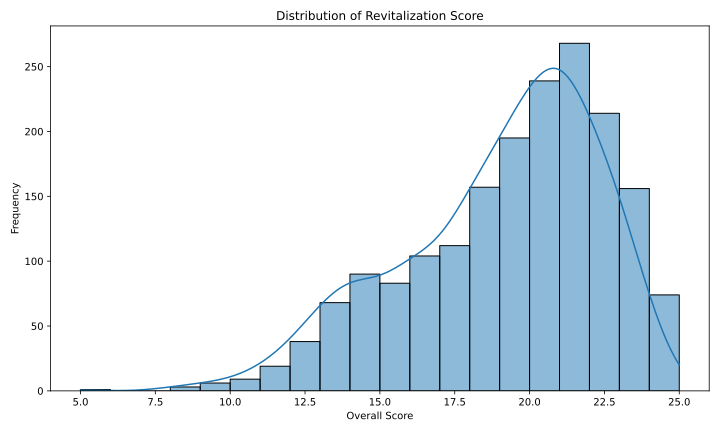
\includegraphics[width=0.8\textwidth]{revitalization_score_distribution.svg}
% \end{figure}

% \begin{figure}[htbp]
%     \centering
%     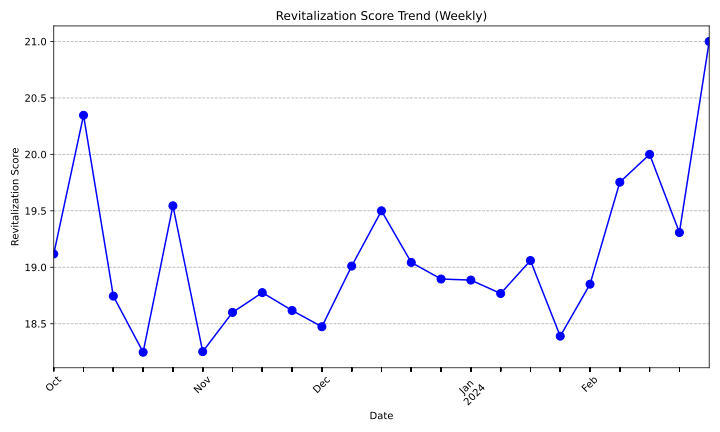
\includegraphics[width=0.8\textwidth]{weekly_revitalization_score_trend.svg}
% \end{figure}

% \begin{figure}[htbp]
%     \centering
%     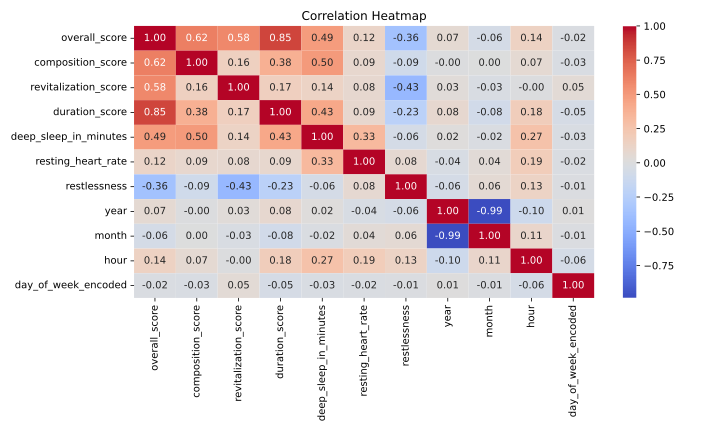
\includegraphics[width=0.8\textwidth]{correlation_heatmap.svg}
% \end{figure}

% \begin{figure}[htbp]
%     \centering
%     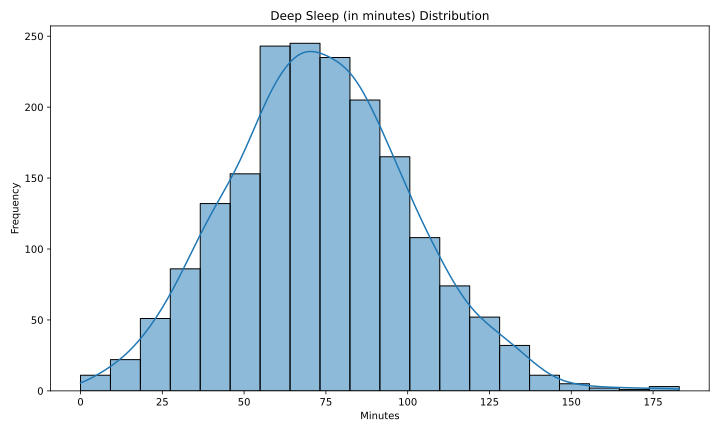
\includegraphics[width=0.8\textwidth]{deep_sleep_distribution.svg}
% \end{figure}

% \begin{figure}[htbp]
%     \centering
%     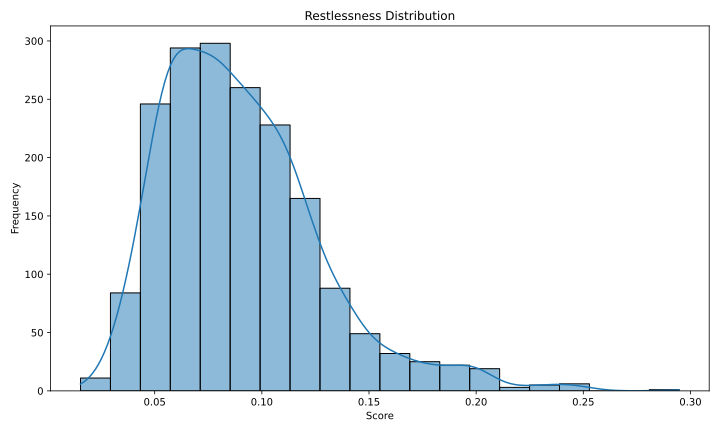
\includegraphics[width=0.8\textwidth]{restlessness_distribution.svg}
% \end{figure}

% \begin{figure}[htbp]
%     \centering
%     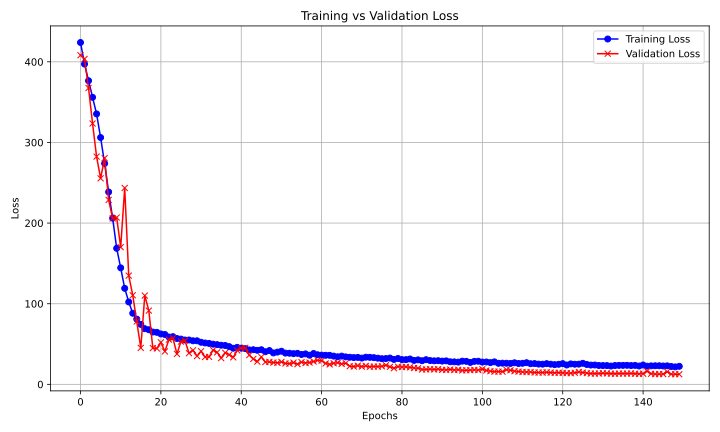
\includegraphics[width=0.8\textwidth]{model_loss_plot.svg}
% \end{figure}

% \begin{figure}[htbp]
%     \centering
%     \includegraphics[width=0.8\textwidth]{model_loss_mae.svg}
% \end{figure}

% \begin{figure}[htbp]
%     \centering
%     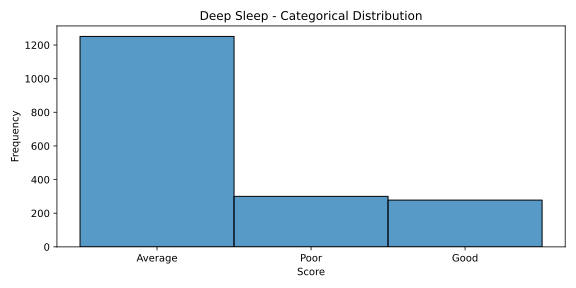
\includegraphics[width=0.8\textwidth]{feature_importance_plot.svg}
% \end{figure}

% \begin{figure}[htbp]
%     \centering
%     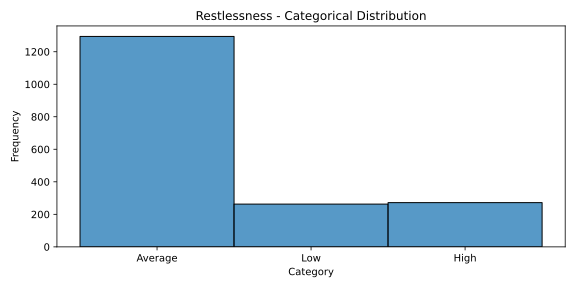
\includegraphics[width=0.8\textwidth]{restlessness_category.svg}
% \end{figure}

% \begin{figure}[htbp]
%     \centering
%     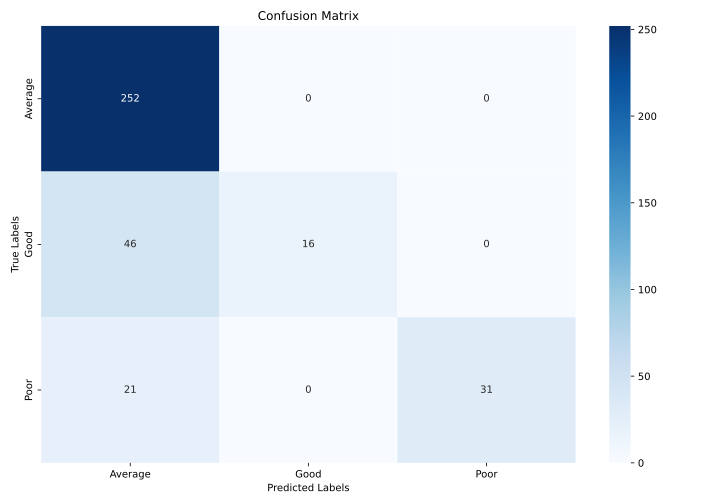
\includegraphics[width=0.8\textwidth]{ml_classifier-confusion_matrix.svg}
% \end{figure}


\subsection{Limitations and Challenges}

The reliance on Fitbit data, while offering a rich source of sleep-related metrics, introduces potential biases associated with wearable device usage, including selection bias and data accuracy concerns.

\subsection{Future Research Directions}

Looking ahead, several avenues for future research emerge from our study. Expanding the dataset to include a broader demographic spectrum and additional physiological parameters could enhance the generalizability and comprehensiveness of the predictive models. Exploring alternative deep learning architectures, such as Convolutional Neural Networks (CNNs) for feature extraction and Recurrent Neural Networks (RNNs) with attention mechanisms, may offer further improvements in model performance. Moreover, integrating environmental and lifestyle variables, such as light exposure, dietary habits, and physical activity levels, could provide a more nuanced understanding of sleep quality determinants.

\subsection{Project Contributions}

Every member equally contributed. Alec and Brandon did most of the AI related tasks and Jon did most of the non-AI related tasks.

\section{Tableau Dashboard}

The dashboard employs a simple and consistent color scheme, with blue as the primary color for all data visualizations. This uniformity helps to avoid visual overload and makes the dashboard aesthetically pleasing while ensuring that users can focus on the data without distraction. Each visualization is clearly labeled with titles, and the axes are marked to ensure that the information is accessible and easily interpreted. This attention to detail supports the dashboard's usability across a broad audience. The layout follows a logical flow, with the most critical information (current status) positioned at the top left, which is typically where a viewer's gaze first lands. This hierarchy of information ensures that the most important data is seen first. The dashboard adopts a minimalist design approach, avoiding unnecessary elements that could clutter the interface. This design choice emphasizes the data itself and supports a more focused user experience.

\newpage

\printbibliography{}

\newpage

\end{document}
